\documentclass[10pt]{article}
\usepackage[utf8]{inputenc}
\usepackage[T1]{fontenc}
\usepackage{amsmath}
\usepackage{amsfonts}
\usepackage{amssymb}
\usepackage[version=4]{mhchem}
\usepackage{stmaryrd}
\usepackage{graphicx}
\usepackage[export]{adjustbox}
\graphicspath{ {./images/} }

\title{Optimization Algorithm for Radiative-Conductive Heat Transfer Model with Boundary Conditions of Cauchy Type $\star \star \star$ }


\author{Alexander Chebotarev ${ }^{1[0000-0002-6456-9138]}$,\\
Andrey Kovtanyuk $2[0000-0002-3286-110 \mathrm{X}]$, and\\
Pavel Mesenev 2[0000-0003-3314-9939]\\
1 Institute for Applied Mathematics FEB RAS, Vladivostok, Russia\\
cheb@iam.dvo.ru\\
2 Far Eastern Federal University, Centre for Research and Education in Mathematics\\
(CREM), Vladivostok, Russia kovtanyuk.ae@dvfu.ru}
\date{}


\begin{document}
\maketitle


\begin{abstract}
To solve the initial boundary-value problem for a quasi-static approximate model of radiative heat transfer, an optimization algorithm is proposed. The analysis of the optimal control problem is carried out, the optimality system is obtained. It is shown that the sequence of solutions of extremal problems converges to the solution of a problem with boundary conditions of Cauchy type for temperature. The results of theoretical analysis are illustrated by numerical examples.
\end{abstract}

Keywords: Equation of radiative heat transfer · Diffusion approximation · Optimal control problem - Cauchy type conditions

\section{Formulation of an Optimal Control Problem}
Quasi-stationary radiative and diffusion heat transfer in a bounded domain $\Omega \subset$ $\mathrm{R}^{3}$ with a boundary $\Gamma=\partial \Omega$ is modeled within the $P_{1}$-approximation for the radiative transfer equation by the following initial-boundary value problem [16, 23]:

$$
\begin{gathered}
\frac{\partial \theta}{\partial t}-a \Delta \theta+b \kappa_{a}\left(|\theta| \theta^{3}-\varphi\right)=0, \\
-\alpha \Delta \varphi+\kappa_{a}\left(\varphi-|\theta| \theta^{3}\right)=0, \quad x \in \Omega, \quad 0<t<T ; \\
a\left(\partial_{n} \theta+\theta\right)=r, \quad \alpha\left(\partial_{n} \varphi+\varphi\right)=u \text { on } \Gamma ; \\
\left.\theta\right|_{t=0}=\theta_{0} .
\end{gathered}
$$

\begin{itemize}
  \item This work was supported by the Russian Foundation for Basic Research (project no. 200100113 (a)) and by the Ministry of Science and Higher Education of the Russian Federation (contract no. 075-02-2020-1482-1, 21.04.2020)
\end{itemize}


\includegraphics[max width=\textwidth, center]{2022_12_28_417a2ab16b2d49239661g-01}
mons License Attribution 4.0 International (CC BY 4.0). Here, $\theta$ is the normalized temperature, $\varphi$ is the normalized intensity of radiation averaged over all directions. The positive parameters $a, b, \kappa_{a}$, and $\alpha$, describing medium properties, are determined by a standard way [18]. The function $r(x, t), x \in \Gamma, t \in(0, T)$ is given, and the unknown function $u(x, t), x \in \Gamma, t \in$ $(0, T)$ is a control. By $\partial_{n}$ we denote the derivative in direction of the outward normal $\mathbf{n}$.

Extremal problem is to find a triple $\left\{\theta_{\lambda}, \varphi_{\lambda}, u_{\lambda}\right\}$ such that

$$
J_{\lambda}(\theta, u)=\frac{1}{2} \int_{0}^{T} \int_{\Gamma}\left(\theta-\theta_{b}\right)^{2} d \Gamma d t+\frac{\lambda}{2} \int_{0}^{T} \int_{\Gamma} u^{2} d \Gamma d t \rightarrow \inf
$$

on solutions of the problem (1)-(3). The function $\theta_{b}(x, t), x \in \Gamma, t \in(0, T)$ and the regularization parameter $\lambda>0$ are given.

The optimal control problem (1)-(4) if $r:=a\left(\theta_{b}+q_{b}\right)$, where $q_{b}$ is a given function on $\Sigma=\Gamma \times(0, T)$, is for small values of $\lambda$ an approximation of the boundary-value problem for equation (1) for which the boundary conditions for the intensity of radiation $\varphi$ are unknown. Instead them the boundary temperature and flow are set,

$$
\left.\theta\right|_{\Gamma}=\theta_{b},\left.\quad \partial_{n} \theta\right|_{\Gamma}=q_{b} .
$$

Mathematical modeling of heat exchange accounting for the radiation effects is used in various applications, e.g., electron microscopic diagnosis [22, 24], glass manufacturing $[13,14]$, and laser thermotherapy [20]. A detailed theoretical and numerical analysis of various formulations of boundary and inverse problems, as well as control problems for the equations of radiation heat transfer within the $P_{1}$-approximation for the radiation transfer equation, is presented in [7$11,16,18,19,23]$. Interesting boundary value problems associated with radiative heat transfer are studied in [2-6]. The nonlocal solvability of nonstationary and steady-state boundary-value problems for the equations of complex heat transfer without boundary conditions on the radiation intensity and with the conditions (5) for temperature is proved in [12].

The main results of the work are to obtain a priori estimates for the solution of the problem (1), (2), on the basis of which the solvability of the optimal control problem (1)-(4) is proved and an optimality system is derived. It is shown that the sequence $\left\{\theta_{\lambda}, \varphi_{\lambda}, u_{\lambda}\right\}$ of solutions to the extremal problem (1)-(4) for $\lambda \rightarrow+0$ converges to the solution of the initial-boundary value problem (1), (5) with conditions of Cauchy type for temperature. An algorithm for solving the control problem is presented.

\section{Formalization of the Control Problem}
In what follows, we assume that $\Omega \subset \mathrm{R}^{3}$ is a bounded strictly Lipschitz domain whose boundary $\Gamma$ consists of a finite number of smooth pieces. By $L^{s}, 1 \leq s \leq$ $\infty$ we denote the Lebesgue space, and by $H^{s}$ the Sobolev space $W_{2}^{s}$. Let $H=$ $L^{2}(\Omega), V=H^{1}(\Omega)$. By $V^{\prime}$ we denote the dual space of $V$, and by $L^{s}(0, T ; X)$ the Lebesgue space of functions from $L^{s}$, defined on $(0, T)$, with values in the space $X$. The space $H$ is identified with the space $H^{\prime}$ so that $V \subset H=H^{\prime} \subset V^{\prime}$. We denote by $\|\cdot\|$ the standard norm in $H$, and by $(f, v)$ the value of the functional $f \in V^{\prime}$ at the element $v \in V$, which coincides with the inner product in $H$ if $f \in H$.

By $U$ we denote the space $L^{2}(\Sigma)$ with the norm

$$
\|u\|_{\Sigma}=\left(\int_{\Sigma} u^{2} d \Gamma d t\right)^{1 / 2} .
$$

We will also use the space $W=\left\{y \in L^{2}(0, T ; V): \quad y^{\prime} \in L^{2}\left(0, T, V^{\prime}\right)\right\}$, where $y^{\prime}=d y / d t$.

We will assume that

(i) $a, b, \alpha, \kappa_{a}, \lambda=$ Const $>0$,

(ii) $\theta_{b}, q_{b} \in U, r=a\left(\theta_{b}+q_{b}\right) \in L^{5}(\Sigma) \theta_{0} \in L^{5}(\Omega)$.

Let us define the operators $A: V \rightarrow V^{\prime}, B: U \rightarrow V^{\prime}$, using the following equalities, which are valid for any $y, z \in V, w \in L^{2}(\Gamma)$ :

$$
(A y, z)=(\nabla y, \nabla z)+\int_{\Gamma} y z d \Gamma, \quad(B w, z)=\int_{\Gamma} w z d \Gamma .
$$

The bilinear form $(A y, z)$ defines the inner product in the space $V$, and the corresponding norm $\|z\|_{V}=\sqrt{(A z, z)}$ is equivalent to the standard norm in $V$. Therefore, the continuous inverse operator is defined $A^{-1}: V^{\prime} \mapsto V$. Note that for any $v \in V, w \in L^{2}(\Gamma), g \in V^{\prime}$ the following inequalities hold:

$$
\|v\|^{2} \leq C_{0}\|v\|_{V}^{2},\|v\|_{V^{\prime}} \leq C_{0}\|v\|_{V},\|B w\|_{V^{\prime}} \leq\|w\|_{\Gamma},\left\|A^{-1} g\right\|_{V} \leq\|g\|_{V^{\prime}} .
$$

Here, the constant $C_{0}>0$ depends only on the domain $\Omega$.

In what follows, we use the following notation $[h]^{s}:=|h|^{s} \operatorname{sign} h, s>0, h \in \mathbf{R}$ for the monotone power function.

Definition. The pair $\theta \in W, \varphi \in L^{2}(0, T ; V)$ is called a weak solution of the problem (1)-(3) if

$$
\theta^{\prime}+a A \theta+b \kappa_{a}\left([\theta]^{4}-\varphi\right)=B r, \quad \theta(0)=\theta_{0}, \quad \alpha A \varphi+\kappa_{a}\left(\varphi-[\theta]^{4}\right)=B u
$$

To formulate the optimal control problem, we define the constraint operator $F(\theta, \varphi, u): W \times L^{2}(0, T ; V) \times U \rightarrow L^{2}\left(0, T, V^{\prime}\right) \times L^{2}\left(0, T, V^{\prime}\right) \times H$ such that

$$
F(\theta, \varphi, u)=\left\{\theta^{\prime}+a A \theta+b \kappa_{a}\left([\theta]^{4}-\varphi\right)-B r, \alpha A \varphi+\kappa_{a}\left(\varphi-[\theta]^{4}\right)-B u, \theta(0)-\theta_{0}\right\} .
$$

Problem $(\mathbf{O C})$. Find the triple $\{\theta, \varphi, u\} \in W \times L^{2}(0, T ; V) \times U$ such that

$$
J_{\lambda}(\theta, u) \equiv \frac{1}{2}\left\|\theta-\theta_{b}\right\|_{\Sigma}^{2}+\frac{\lambda}{2}\|u\|_{\Sigma}^{2} \rightarrow \inf , \quad F(\theta, \varphi, u)=0 .
$$

\section{Solvability of the Problem (OC)}
Let us first prove the unique solvability of the problem (1)-(3).

Lemma 1. Let conditions (i), (ii), $u \in U$ hold. Then there is a unique weak solution to the problem (1)-(3) and, moreover,

$$
\psi=[\theta]^{5 / 2} \in L^{\infty}(0, T ; H) \cap L^{2}(0, T ; V), \quad[\theta]^{4} \in L^{2}(0, T ; H) .
$$

Proof. Let us express $\varphi$ from the last equation of (6) and substitute it into the first one. As a result, we obtain the following Cauchy problem for an equation with operator coefficients:

$$
\theta^{\prime}+a A \theta+L[\theta]^{4}=B r+f, \quad \theta(0)=\theta_{0} .
$$

Here,

$$
L=\alpha b \kappa_{a} A\left(\alpha A+\kappa_{a} I\right)^{-1}: V^{\prime} \rightarrow V^{\prime}, f=b \kappa_{a}\left(\alpha A+\kappa_{a} I\right)^{-1} B u \in L^{2}(0, T ; V) .
$$

Let us obtain a priori estimates for the solution of the problem (7), on the basis of which the solvability of this problem is derived in a standard way. Let $[\zeta, \eta]=\left(\left(\alpha I+\kappa_{a} A^{-1}\right) \zeta, \eta\right), \zeta \in V^{\prime}, \eta \in V$. Note that the expression $[[\eta]]=\sqrt{[\eta, \eta]}$ defines the norm in $H$ equivalent to the standard one.

Multiplying, in the sense of the inner product of $H$, the equation in (7) by $\left(\alpha I+\kappa_{a} A^{-1}\right) \theta$, we obtain

$$
\frac{1}{2} \frac{d}{d t}[[\theta]]^{2}+a \alpha(A \theta, \theta)+a \kappa_{a}\|\theta\|^{2}+\alpha b \kappa_{a}\|\theta\|_{L^{5}(\Omega)}^{5}=[B r, \theta]+[f, \theta] .
$$

The equality (8) implies the estimate

$$
\|\theta\|_{L^{\infty}(0, T ; H)}+\|\theta\|_{L^{2}(0, T ; V)}+\|\theta\|_{L^{5}(Q)} \leq C_{1},
$$

where $C_{1}$ depends only on $a, b, \alpha, \kappa_{a},\|f\|_{L^{2}(0, T ; H)},\left\|\theta_{0}\right\|,\|r\|_{L^{2}(\Sigma)}$.

Further, let $\psi=[\theta]^{5 / 2}$. Note that

$$
\left(\theta^{\prime},[\theta]^{4}\right)=\frac{1}{5} \frac{d}{d t}\|\psi\|^{2}, \quad\left(A \theta,[\theta]^{4}\right)=\frac{16}{25}\|\nabla \psi\|^{2}+\|\psi\|_{L^{2}(\Gamma)}^{2} .
$$

Multiplying, in the sense of the inner product of $H$, the equation in (7) by $[\theta]^{4}=[\psi]^{8 / 5}$, we obtain

$$
\frac{1}{5} \frac{d}{d t}\|\psi\|^{2}+a\left(\frac{16}{25}\|\nabla \psi\|^{2}+\|\psi\|_{L^{2}(\Gamma)}^{2}\right)+\left(L[\psi]^{8 / 5},[\psi]^{8 / 5}\right)=\left(B r+f,[\psi]^{8 / 5}\right) .
$$

The equality (10) implies the estimate

$$
\|\psi\|_{L^{\infty}(0, T ; H)}+\|\psi\|_{L^{2}(0, T ; V)}+\left\|[\theta]^{4}\right\|_{L^{2}(0, T ; H)} \leq C_{2},
$$

where $C_{2}$ depends only on $a, b, \alpha, \kappa_{a},\|f\|_{L^{2}(0, T ; H)},\left\|\theta_{0}\right\|_{L^{5}(\Omega)},\|r\|_{L^{5}(\Sigma)}$. Further, let us estimate $\left\|\theta^{\prime}\right\|_{L^{2}\left(0, T ; V^{\prime}\right)}$ taking into account $\theta^{\prime}=B r+f-a A \theta-L[\theta]^{4}$. Due to the conditions on the initial data, it is true that $B r, f \in L^{2}\left(0, T ; V^{\prime}\right)$. Since $\theta \in L^{2}(0, T ; V)$, then $A \theta \in L^{2}\left(0, T ; V^{\prime}\right)$. Let $\zeta=L[\theta]^{4}$. Then

$$
\alpha \zeta+\kappa_{a} A^{-1} \zeta=\alpha b \kappa_{a}[\theta]^{4} .
$$

Multiplying, in the sense of the inner product of $H$, the last equality by $\zeta$, we obtain

$$
\alpha\|\zeta\|^{2}+\kappa_{a}\left(A^{-1} \zeta, \zeta\right)=\alpha b \kappa_{a}\left([\theta]^{4}, \zeta\right) \leq \alpha\left(\|\zeta\|^{2}+\frac{\left(b \kappa_{a}\right)^{2}}{4}\left\|[\theta]^{4}\right\|^{2}\right) \text {. }
$$

Therefore, $\|\zeta\|_{V^{\prime}}^{2}=\left(A^{-1} \zeta, \zeta\right) \leq \frac{\alpha \kappa_{a} b^{2}}{4}\left\|[\theta]^{4}\right\|^{2}$ and, by virtue of the estimates (9), (11), we obtain

$$
\left\|\theta^{\prime}\right\|_{L^{2}\left(0, T ; V^{\prime}\right)} \leq\|B r+f\|_{L^{2}\left(0, T ; V^{\prime}\right)}+a C_{1}+\sqrt{\alpha \kappa_{a}} b C_{2} .
$$

The estimates (9)-(12) are sufficient to prove the solvability of the problem.

Let $\theta_{1,2}$ be solutions of the problem (7), $\eta=\theta_{1}-\theta_{2}$. Then

$$
\eta^{\prime}+a A \eta+L\left(\left[\theta_{1}\right]^{4}-\left[\theta_{1}\right]^{4}\right)=0, \quad \eta(0)=0 .
$$

Multiplying, in the sense of the inner product of $H$, the last equation by $\left(\alpha I+\kappa_{a} A^{-1}\right) \eta$, we obtain

$$
\frac{1}{2} \frac{d}{d t}[[\eta]]^{2}+a \alpha(A \eta, \eta)+a \kappa_{a}\|\eta\|^{2}+\alpha b \kappa_{a}\left(\left[\theta_{1}\right]^{4}-\left[\theta_{1}\right]^{4}, \theta_{1}-\theta_{2}\right)=0 .
$$

The last term on the left-hand side is non-negative and therefore, integrating the resulting equality over time, we derive $\eta=\theta_{1}-\theta_{2}=0$, which means the uniqueness of the solution. The lemma is proved.

Theorem 1. Let conditions (i), (ii) hold. Then there is a solution of the problem $(O C)$.

Proof. Let $j_{\lambda}=\inf J_{\lambda}$ on the set $u \in U, F(\theta, \varphi, u)=0$. We choose a minimizing sequence $u_{m} \in U, \theta_{m} \in W, \varphi_{m} \in L^{2}(0, T ; V), J_{\lambda}\left(\theta_{m}, u_{m}\right) \rightarrow j_{\lambda}$,

$$
\begin{aligned}
\theta_{m}^{\prime}+a A \theta_{m}+b \kappa_{a}\left(\left[\theta_{m}\right]^{4}-\varphi_{m}\right)=B r, & \theta_{m}(0)=\theta_{0}, \\
& \alpha A \varphi_{m}+\kappa_{a}\left(\varphi_{m}-\left[\theta_{m}\right]^{4}\right)=B u_{m} .
\end{aligned}
$$

The boundedness of the sequence $u_{m}$ in the space $U$ implies, by Lemma 1 , the estimates

$$
\begin{gathered}
\left\|\theta_{m}\right\|_{L^{2}(0, T ; V)} \leq C, \quad\left\|\theta_{m}\right\|_{L^{\infty}\left(0, T ; L^{5}(\Omega)\right)} \leq C,\left\|\theta_{m}^{\prime}\right\|_{L^{2}\left(0, T ; V^{\prime}\right)} \leq C, \\
\int_{0}^{T} \int_{\Omega}\left|\theta_{m}\right|^{8} d x d t \leq C, \quad\left\|\varphi_{m}\right\|_{L^{2}(0, T ; V)} \leq C .
\end{gathered}
$$

Here, $C>0$ denotes the largest of the constants limiting the corresponding norms and not depending on $m$. Passing, if necessary, to subsequences, we conclude that there is a triple $\{\widehat{u}, \widehat{\theta}, \widehat{\varphi}\} \in U \times W \times L^{2}(0, T ; V)$,

$$
\begin{gathered}
u_{m} \rightarrow \widehat{u} \text { weakly in } U \\
\theta_{m} \rightarrow \widehat{\theta} \text { weakly in } L^{2}(0, T ; V), \text { strongly in } L^{2}(Q), \\
\varphi_{m} \rightarrow \widehat{\varphi} \text { weakly in } L^{2}(0, T ; V) .
\end{gathered}
$$

Moreover, $\widehat{\theta} \in L^{8}(Q) \cap L^{\infty}\left(0, T ; L^{5}(\Omega)\right)$.

Convergence results allow us to pass to the limit in (13). In this case, the passage to the limit in the nonlinear terms follows from the following inequality, which is valid for $\xi \in C^{\infty}(\bar{Q})$ :

$$
\begin{aligned}
& \int_{0}^{T}\left|\left(\left[\theta_{m}\right]^{4}-[\widehat{\theta}]^{4}, \xi\right)\right| d t \leq \\
& \quad 2 \max _{\bar{Q}}|\xi|\left(\left\|\theta_{m}\right\|_{L^{5}(\Omega)}^{5 / 3}\left\|\theta_{m}\right\|_{L^{8}(\Omega)}^{4 / 3}+\|\widehat{\theta}\|_{L^{5}(\Omega)}^{5 / 3}\|\widehat{\theta}\|_{L^{8}(\Omega)}^{4 / 3}\right)\left\|\theta_{m}-\widehat{\theta}\right\|_{L^{2}(Q)} .
\end{aligned}
$$

Therefore,

$$
\widehat{\theta}^{\prime}+a A \widehat{\theta}+b \kappa_{a}\left([\widehat{\theta}]^{4}-\widehat{\varphi}\right)=B r, \quad \widehat{\theta}(0)=\theta_{0}, \quad \alpha A \widehat{\varphi}+\kappa_{a}\left(\widehat{\varphi}-[\widehat{\theta}]^{4}\right)=B \widehat{u},
$$

and wherein $j_{\lambda} \leq J_{\lambda}(\widehat{\theta}, \widehat{u}) \leq \underline{\lim } J_{\lambda}\left(\theta_{m}, u_{m}\right)=j_{\lambda}$. Thus, the triple $\{\widehat{\theta}, \widehat{\varphi}, \widehat{u}\}$ is a solution of the problem $(O C)$.

\section{Optimality Conditions}
To obtain an optimality system, it is sufficient to use the Lagrange principle for smooth-convex extremal problems [15,17]. Let us check the validity of the key condition that the image of the derivative of the constraint operator $F_{y}^{\prime}(y, u)$, where $y=\{\theta, \varphi\} \in W \times L^{2}(0, T ; V)$, coincides with space $L^{2}\left(0, T ; V^{\prime}\right) \times L^{2}\left(0, T ; V^{\prime}\right) \times H$. It is this condition that guarantees the nondegeneracy of the optimality conditions. Recall that

$F(\theta, \varphi, u)=\left\{\theta^{\prime}+a A \theta+b \kappa_{a}\left([\theta]^{4}-\varphi\right)-B r, \alpha A \varphi+\kappa_{a}\left(\varphi-[\theta]^{4}\right)-B u, \theta(0)-\theta_{0}\right\}$.

Lemma 2. Let the conditions (i), (ii) hold. If $\widehat{y} \in W \times L^{2}(0, T ; V), \widehat{u} \in U$ is a solution of the problem (OC), then the following equality is valid:

$$
\operatorname{Im} F_{y}^{\prime}(\widehat{y}, \widehat{u})=L^{2}\left(0, T ; V^{\prime}\right) \times L^{2}\left(0, T ; V^{\prime}\right) \times H .
$$

Proof. It is enough to check that the problem

$$
\xi^{\prime}+a A \xi+b \kappa_{a}\left(4|\widehat{\theta}|^{3} \xi-\eta\right)=f_{1}, \quad \xi(0)=\xi_{0}, \quad \alpha A \eta+\kappa_{a}\left(\eta-4|\widehat{\theta}|^{3} \xi\right)=f_{2}
$$

is solvable for all $f_{1,2} \in L^{2}\left(0, T ; V^{\prime}\right), \xi_{0} \in H$. Let us express $\eta$ from the last equation and substitute it into the first one. As a result, we get the following problem:

$$
\xi^{\prime}+a A \xi+4 L\left(|\widehat{\theta}|^{3} \xi\right)=f_{1}+b \kappa_{a}\left(\alpha A+\kappa_{a} I\right)^{-1} f_{2}, \xi(0)=\xi_{0} .
$$

The unique solvability of the linear problem (14) is proved similarly to Lemma 1. According to Lemma 2, the Lagrangian of the problem (OC) has the form

$$
\begin{aligned}
& L\left(\theta, \varphi, u, p_{1}, p_{2}, q\right)=J_{\lambda}(\theta, u)+\int_{0}^{T}\left(\theta^{\prime}+a A \theta+b \kappa_{a}\left([\theta]^{4}-\varphi\right)-B r, p_{1}\right) d t \\
&+\int_{0}^{T}\left(\alpha A \varphi+\kappa_{a}\left(\varphi-[\theta]^{4}\right)-B u, p_{2}\right) d t+\left(q, \theta(0)-\theta_{0}\right) .
\end{aligned}
$$

Here, $p=\left\{p_{1}, p_{2}\right\} \in L^{2}(0, T ; V) \times L^{2}(0, T ; V)$ Is the conjugate state, $q \in H$ is the Lagrange multiplier for the initial condition. If $\{\widehat{\theta}, \widehat{\varphi}, \widehat{u}\}$ is a solution of the problem (OC), then by virtue of the Lagrange principle [15, Ch. 2, Theorem 1.5] the variational equalities hold $\forall \zeta \in L^{2}(0, T ; V), v \in U$

$$
\begin{gathered}
\int_{0}^{T}\left(\left(B\left(\widehat{\theta}-\theta_{b}\right), \zeta\right)+\left(\zeta^{\prime}+a A \zeta+4 b \kappa_{a}|\widehat{\theta}|^{3} \zeta, p_{1}\right)-\kappa_{a}\left(4|\widehat{\theta}|^{3} \zeta, p_{2}\right)\right) d t+(q, \zeta(0))=0, \\
\int_{0}^{T}\left(\left(\alpha A \zeta+\kappa_{a} \zeta, p_{2}\right)-b \kappa_{a}\left(\zeta, p_{1}\right)\right) d t=0, \int_{0}^{T}\left(\lambda(\widehat{u}, v)_{\Gamma}-\left(B v, p_{2}\right)\right) d t=0 .
\end{gathered}
$$

Thus, from the obtained conditions, we derive the following result.

Theorem 2. Let the conditions (i),(ii) hold. If $\{\widehat{\theta}, \widehat{\varphi}, \widehat{u}\}$ is a solution of the problem $(O C)$, then there is a unique pair $\left\{p_{1}, p_{2}\right\} \in W \times W$ such that

$$
\begin{aligned}
-p_{1}^{\prime}+a A p_{1}+4|\widehat{\theta}|^{3} \kappa_{a}\left(b p_{1}-p_{2}\right)=B\left(\theta_{b}-\widehat{\theta}\right), & p_{1}(T)=0, \\
& \alpha A p_{2}+\kappa_{a}\left(p_{2}-b p_{1}\right)=0
\end{aligned}
$$

and wherein $\lambda \widehat{u}=\left.p_{2}\right|_{\Sigma}$.

\section{Approximation of a Problem with Boundary Conditions of Cauchy Type}
Let us consider an initial-boundary value problem for the equations of complex heat transfer, in which there are no boundary conditions on the radiation intensity:

$$
\frac{\partial \theta}{\partial t}-a \Delta \theta+b \kappa_{a}\left([\theta]^{4}-\varphi\right)=0, \quad-\alpha \Delta \varphi+\kappa_{a}\left(\varphi-[\theta]^{4}\right)=0, \quad(x, t) \in Q,
$$

$$
\theta=\theta_{b}, \quad \partial_{n} \theta=q_{b} \text { on } \Sigma,\left.\quad \theta\right|_{t=0}=\theta_{0} .
$$

Existence and uniqueness of functions $\theta \in L^{2}\left(0, T ; H^{2}(\Omega)\right), \varphi, \Delta \varphi \in L^{2}(Q)$, satisfying (16), (17) for sufficiently smooth $\theta_{b}, q_{b}$ are proved in [12]. Let us show that solutions of the problem (OC) for $\lambda \rightarrow+0$ approximate the solution of the problem $(16),(17)$

Theorem 3. Let the conditions (i),(ii) hold and there is a solution $\theta, \varphi \in$ $L^{2}\left(0, T ; H^{2}(\Omega)\right)$ of the problem (16), (17). If $\left\{\theta_{\lambda}, \varphi_{\lambda}, u_{\lambda}\right\}$ is a solution of the problem $(O C)$ for $\lambda>0$, then as $\lambda \rightarrow+0$

$$
\begin{gathered}
\theta_{\lambda} \rightarrow \theta \text { weakly in } L^{2}(0, T ; V), \text { strongly in } L^{2}(Q), \\
\varphi_{\lambda} \rightarrow \varphi \text { weakly in } L^{2}(0, T ; V)
\end{gathered}
$$

Proof. Let $\theta, \varphi \in L^{2}\left(0, T ; H^{2}(\Omega)\right)$ be a solution of the problem $(16),(17), u=$ $\alpha\left(\partial_{n} \varphi+\varphi\right) \in U$. Then

$$
\theta^{\prime}+a A \theta+b \kappa_{a}\left([\theta]^{4}-\varphi\right)=B r, \quad \theta(0)=\theta_{0}, \quad \alpha A \varphi+\kappa_{a}\left(\varphi-[\theta]^{4}\right)=B u
$$

where $r:=a\left(\theta_{b}+q_{b}\right)$. Therefore, taking into account that $\left.\theta\right|_{\Gamma}=\theta_{b}$,

$$
J_{\lambda}\left(\theta_{\lambda}, u_{\lambda}\right)=\frac{1}{2}\left\|\theta_{\lambda}-\theta_{b}\right\|_{\Sigma}^{2}+\frac{\lambda}{2}\left\|u_{\lambda}\right\|_{\Sigma}^{2} \leq J_{\lambda}(\theta, u)=\frac{\lambda}{2}\|u\|_{\Sigma}^{2} .
$$

Thus,

$$
\left\|u_{\lambda}\right\|_{\Sigma}^{2} \leq C, \quad\left\|\theta_{\lambda}-\theta_{b}\right\|_{\Sigma}^{2} \rightarrow 0, \lambda \rightarrow+0 .
$$

Hereinafter, $C>0$ does not depend on $\lambda$. The boundedness of the sequence $u_{\lambda}$ in the space $U$ implies, by Lemma 1 , the estimates

$$
\begin{gathered}
\left\|\theta_{\lambda}\right\|_{L^{2}(0, T ; V)} \leq C, \quad\left\|\theta_{\lambda}\right\|_{L^{\infty}\left(0, T ; L^{5}(\Omega)\right)} \leq C, \quad\left\|\theta_{\lambda}^{\prime}\right\|_{L^{2}\left(0, T ; V^{\prime}\right)} \leq C, \\
\int_{0}^{T} \int_{\Omega}\left|\theta_{\lambda}\right|^{8} d x d t \leq C, \quad\left\|\varphi_{\lambda}\right\|_{L^{2}(0, T ; V)} \leq C .
\end{gathered}
$$

Therefore, one can choose a sequence $\lambda \rightarrow+0$ such that

$$
\begin{gathered}
u_{\lambda} \rightarrow u_{*} \text { weakly in } U \\
\theta_{\lambda} \rightarrow \theta_{*} \text { weakly in } L^{2}(0, T ; V) \text {, strongly in } L^{2}(Q), \\
\varphi_{\lambda} \rightarrow \varphi_{*} \text { weakly in } L^{2}(0, T ; V)
\end{gathered}
$$

The obtained results on convergence allow, as in Theorem 1 , to pass to the limit as $\lambda \rightarrow+0$ in the equations for $\theta_{\lambda}, \varphi_{\lambda}, u_{\lambda}$ and then

$\theta_{*}^{\prime}+a A \theta_{*}+b \kappa_{a}\left(\left[\theta_{*}\right]^{4}-\varphi_{*}\right)=B r, \quad \theta_{*}(0)=\theta_{0}, \quad \alpha A \varphi_{*}+\kappa_{a}\left(\varphi_{*}-\left[\theta_{*}\right]^{4}\right)=B u_{*}$. Wherein $\left.\theta_{*}\right|_{\Gamma}=\theta_{b}$. From the first equation in (18), taking into account that $r=a\left(\theta_{b}+q_{b}\right)$, we derive

$$
\frac{\partial \theta_{*}}{\partial t}-a \Delta \theta_{*}+b \kappa_{a}\left(\left[\theta_{*}\right]^{4}-\varphi_{*}\right)=0 \text { a.e. in } Q, \quad \theta_{*}=\theta_{b}, \quad \partial_{n} \theta=q_{b} \text { a.e. in } \Sigma \text {. }
$$

From the second equation in (18) it follows that $-\alpha \Delta \varphi+\kappa_{a}\left(\varphi-[\theta]^{4}\right)=0$ almost everywhere in $Q$. Thus, the pair $\theta_{*}, \varphi_{*}$ is a solution of the problem (16), (17). Since the solution to this problem is unique [12], then $\theta_{*}=\theta, \varphi_{*}=\varphi$.

\section{Numerical Algorithm and Examples}
Let us present an algorithm for solving the control problem. Let

$$
\widetilde{J}_{\lambda}(u)=J_{\lambda}(\theta(u), u),
$$

where $\theta(u)$ is the component of solution to the problem (1)-(2) corresponding to the control $u \in U$. According to (15), the gradient of the functional $\widetilde{J}_{\lambda}(u)$ is defined as follows: $\widetilde{J}_{\lambda}^{\prime}(u)=\lambda u-p_{2}$. Here, $p_{2}$ is the corresponding component of the conjugate state of the system (15), where $\widehat{\theta}:=\theta(u)$.

The proposed algorithm for solving the problem (OC) is as follows:

Algorithm 1 Gradient descent algorithm

1: Choosing the value of the gradient step $\varepsilon$,

2: Choosing the number of iterations $N$,

3: Choosing an initial approximation for the control $u_{0} \in U$,

4: for $k \leftarrow 0,1,2, \ldots, N$ do :

5: $\quad$ For a given $u_{k}$, calculate the state $y_{k}=\left\{\theta_{k}, \varphi_{k}\right\}$, a solution of the problem (1)-(3).

6: $\quad$ We calculate the value of the quality functional $J_{\lambda}\left(\theta_{k}, u_{k}\right)$.

7: From equations (15), we calculate the conjugate state $p_{k}=\left\{p_{1 k}, p_{2 k}\right\}$, where $\widehat{\theta}:=\theta_{k}, \widehat{u}:=u_{k}$.

8: $\quad$ We We recalculate the control $u_{k+1}=u_{k}-\varepsilon\left(\lambda u_{k}-p_{2}\right)$

The parameter $\varepsilon$ is chosen empirically so that the value of $\varepsilon\left(\lambda u_{k}-p_{2}\right)$ is a significant correction for $u_{k+1}$. The number of iterations $N$ is chosen sufficient to satisfy the condition $J_{\lambda}\left(\theta_{k}, u_{k}\right)-J_{\lambda}\left(\theta_{k+1}, u_{k+1}\right)<\delta$, where $\delta>0$ determines the accuracy of the calculations.

The example considered below illustrates the performance of the proposed algorithm for small, which is important, values of the regularization parameter $\lambda \leq 10^{-12}$. Note that for the numerical solution of a direct problem with a given control, the simple iteration method was used to linearize the problem and solve it by the finite element method. Solving a conjugate system that is linear at a given temperature is straightforward. For numerical simulation, we used the solver FEniCS [1,21]. Let us compare the work of the proposed algorithm with the results of the article [12]. The problem is considered in the domain $\Omega \times(-L, L)$, where $\Omega=$ $\left\{x=\left(x_{1}, x_{2}\right): 0<x_{1,2}<d\right\}$ and for large $L$ reduces to a two-dimensional problem for the computational domain $\Omega$. The following values of the problem parameters were chosen: $d=1(\mathrm{~m}), a=0.9210^{-4}\left(\mathrm{~m}^{2} / \mathrm{s}\right), b=0.19(\mathrm{~m} / \mathrm{s})$, $\alpha=0.0333(\mathrm{~m}) \quad \kappa_{a}=1\left(\mathrm{~m}^{-1}\right)$. The parameters correspond to air at normal atmospheric pressure and temperature $400^{\circ} \mathrm{C}$. The function $\theta_{b}, q_{b}$ for the boundary condition (5) are set as follows: $\theta_{b}=\left.\widehat{\theta}\right|_{\Gamma}, q_{b}=\left.\partial_{n} \widehat{\theta}\right|_{\Gamma}$, where $\widehat{\theta}=$ $\left(x_{1}-0.5\right)^{2}-0.5 x_{2}+0.75$.

An approximate solution to the problem (16), (17) with Cauchy data, presented in [12] (see Fig. 1), was obtained by solving a fourth-order parabolic problem for temperature.

\begin{center}
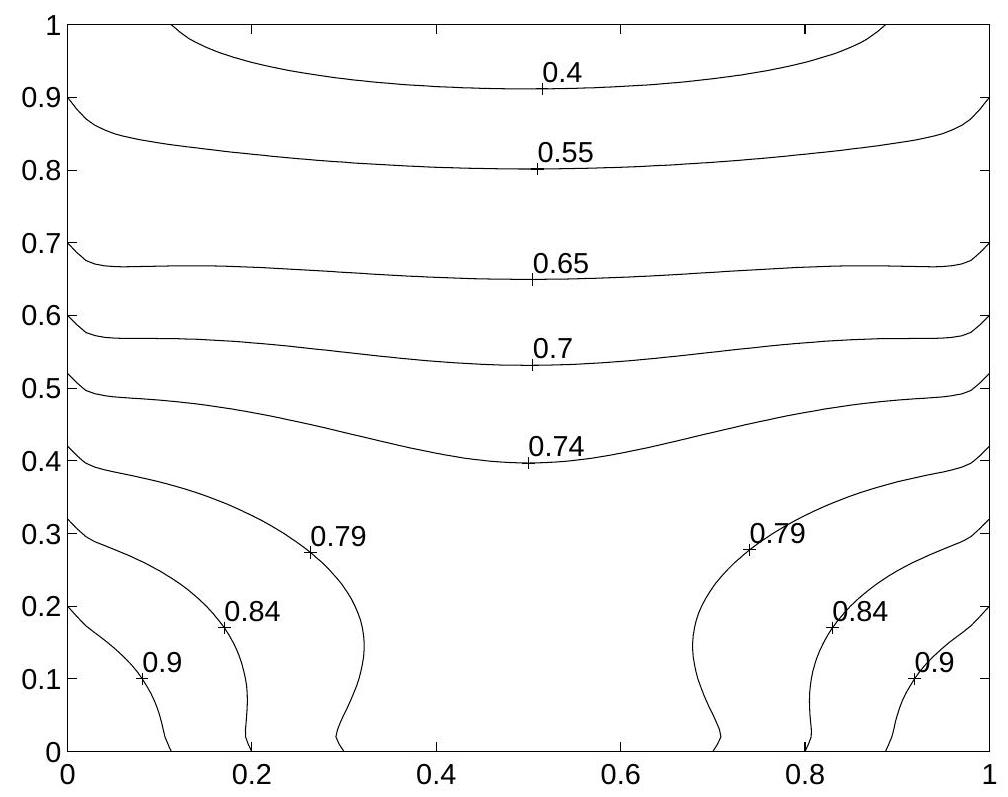
\includegraphics[max width=\textwidth]{2022_12_28_417a2ab16b2d49239661g-10}
\end{center}

Fig. 1. Temperature field obtained in the article [12].

The solution stabilized after 120 seconds, but the calculations at each time step were quite expensive [12]. Fig. 2 shows the steady-state temperature field obtained by the method proposed in the current article.

The presented example illustrates that the proposed algorithm successfully finds a numerical solution to the problem (16), (17) with the boundary conditions of the Cauchy type.

\begin{center}
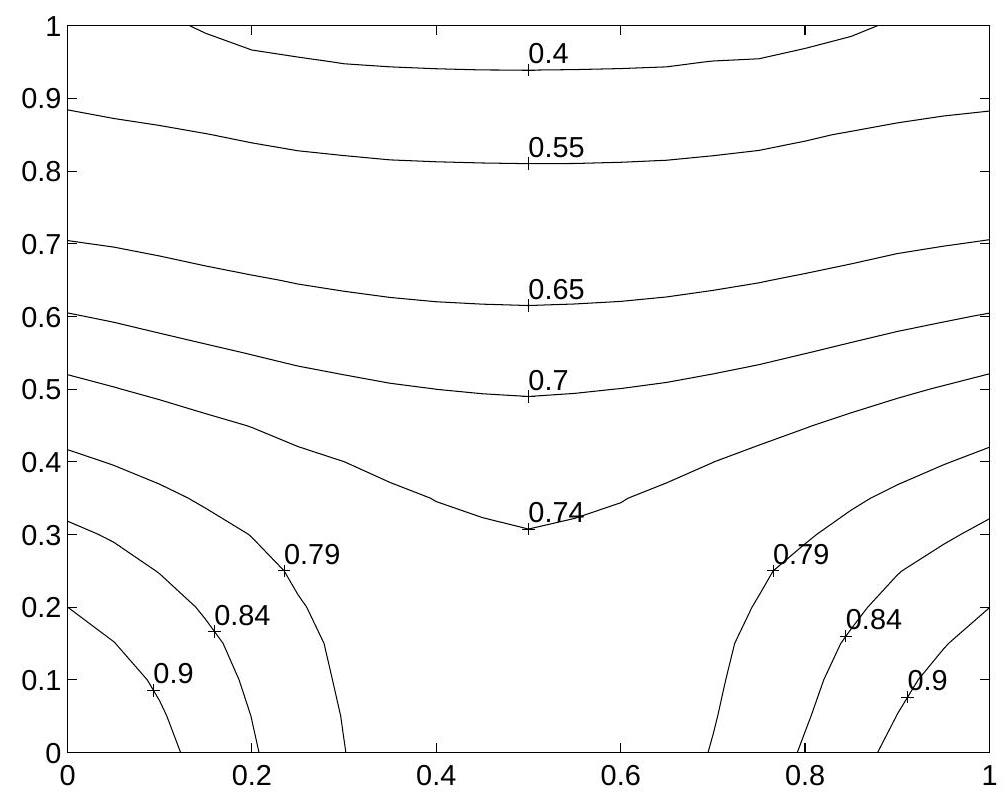
\includegraphics[max width=\textwidth]{2022_12_28_417a2ab16b2d49239661g-11}
\end{center}

Fig. 2. Temperature field obtained by the proposed algorithm.

\section{References}
\begin{enumerate}
  \item Alnaes, M.S., Blechta, J., Hake, J., Johansson, A., Kehlet, B., Logg, A., Richardson, C., Ring, J., Rognes, M.E., Wells, G.N.: The FEniCS project version 1.5. Archive of Numerical Software 3(100), 9-23 (2015)

  \item Amosov, A.A.: Stationary nonlinear nonlocal problem of radiative-conductive heat transfer in a system of opaque bodies with properties depending on the radiation frequency. J. Math. Sci. 164(3), 309-344 (2010)

  \item Amosov, A.A.: Unique solvability of a nonstationary problem of radiativeconductive heat exchange in a system of semitransparent bodies. Russian J. of Math. Phys. 23 $(3), 309-334(2016)$

  \item Amosov, A.A.: Unique solvability of stationary radiative-conductive heat transfer problem in a system of semitransparent bodies. J. Math. Sci. $\mathbf{2 2 4}(5), 618-646$ $(2017)$

  \item Amosov, A.A.: Asymptotic behavior of a solution to the radiative transfer equation in a multilayered medium with diffuse reflection and refraction conditions. J. Math. Sci. 244, 541-575 (2020)

  \item Amosov, A.A., Krymov, N.E.: On a nonstandard boundary value problem arising in homogenization of complex heat transfer problems. J. Math. Sci. 244, 357-377 $(2020)$

  \item Chebotarev, A.Yu., Kovtanyuk, A.E., Grenkin, G.V., Botkin, N.D., Hoffmann, K.-H.: Nondegeneracy of optimality conditions in control problems for a radiative-conductive heat transfer model. Appl. Math. Comput. 289, 371-380 (2016) 8. Chebotarev, A.Yu., Grenkin, G.V., Kovtanyuk, A.E.: Inhomogeneous steady-state problem of complex heat transfer. ESAIM Math. Model. Numer. Anal. 51(6), 2511-2519 (2017)

  \item Chebotarev, A.Y., Grenkin, G.V., Kovtanyuk, A.E., Botkin, N.D., Hoffmann, K.-H.: Diffusion approximation of the radiative-conductive heat transfer model with Fresnel matching conditions. Comm. Nonlin. Sci. Num. Simulat. 57, 290-298 (2018)

  \item Chebotarev, A.Yu., Grenkin, G.V., Kovtanyuk, A.E., Botkin, N.D., Hoffmann, K.-H.: Inverse problem with finite overdetermination for steadystate equations of radiative heat exchange. J. Math. Anal. Appl. 460(2), 737-744 $(2018)$

  \item Chebotarev, A.Yu., Pinnau, R.: An inverse problem for a quasi-static approximate model of radiative heat transfer. J. Math. Anal. Appl. 472(1), 314-327 (2019)

  \item Chebotarev, A.Y., Kovtanyuk, A.E., Botkin, N.D.: Problem of radiation heat exchange with boundary conditions of the Cauchy type. Comm. Nonlin. Sci. Num. Simulat. 75, 262-269 (2019)

  \item Clever, D., Lang, J.: Optimal control of radiative heat transfer in glass cooling with restrictions on the temperature gradient. Optimal Control Appl. Meth. 33(2), 157-175 (2012)

  \item Frank, M., Klar, A., Pinnau, R.: Optimal control of glass cooling using simplified PN theory. Trans. Theory Stat. Phys. 39(2-4), 282-311 (2010)

  \item Fursikov, A.V.: Optimal control of distributed systems. Theory and applications. American Math. Soc., Providence, Rhode Island (2000)

  \item Grenkin, G.V., Chebotarev, A.Yu., Kovtanyuk, A.E., Botkin, N.D., Hoffmann, K.-H.: Boundary optimal control problem of complex heat transfer model. J. Math. Anal. Appl. 433(2), 1243-1260 (2016)

  \item Ioffe, A.D., Tikhomirov, V.M.: Theory of extremal problems. North-Holland, Amsterdam (1979)

  \item Kovtanyuk, A.E., Chebotarev, A.Yu., Botkin, N.D., Hoffmann, K.-H.: Unique solvability of a steady-state complex heat transfer model. Commun. Nonlinear Sci. Numer. Simul. 20(3), 776-784 (2015)

  \item Kovtanyuk, A.E., Chebotarev, A.Yu., Botkin, N.D., Hoffmann, K.-H.: Optimal boundary control of a steady-state heat transfer model accounting for radiative effects. J. Math. Anal. Appl. 439(2), 678-689 (2016)

  \item Kovtanyuk, A.E., Chebotarev, A.Yu., Astrakhantseva, A.A., Sushchenko, A.A.: Optimal control of endovenous laser ablation. Optics and Spectroscopy 128(9), 1508-1516 (2020)

  \item Logg, A., Wells, G.N.: DOLFIN: Automated Finite Element Computing. ACM Trans. Math. Software. $\mathbf{3 7}(2), 20$ (2010)

  \item Maslovskaya, A., Pavelchuk, A.: Simulation of heat conductivity and charging processes in polar dielectrics induced by electron beam exposure. IOP Conf. Series: Materials Sci. Eng. 81(1), 012119 (2015)

  \item Pinnau, R.: Analysis of optimal boundary control for radiative heat transfer modeled by $\mathrm{SP}_{1}$-system. Commun. Math. Sci. 5(4), 951-969 (2007)

  \item Sogr, A.A., Maslovskaya, A.G.: Estimation of SEM imaging resolution of the domain structure of pyroprobe-heated ferroelectrics. Tech. Phys. 49(11), 1505-1508 (2004)

\end{enumerate}

\end{document}